\documentclass[11pt, a4paper]{article}
\usepackage[T1]{fontenc}
\usepackage[utf8]{inputenc}
\usepackage[french]{babel}
\usepackage{hyperref}
\usepackage{graphicx}      
\usepackage{xcolor}        
\usepackage[acronym]{glossaries}
\usepackage{fancyhdr}
\usepackage{url}
\Urlmuskip=0mu plus 1mu
\pagestyle{fancy}
\fancyhf{}
\fancyhead[L]{\raisebox{-3pt}{\rule{\textwidth}{0.4pt}}}
\fancyhead[R]{\raisebox{3pt}{\textbf{Solitude 408}}}
\fancyfoot[L]{
  \raisebox{3pt}{
    \begin{tabular}{l}
      Louay Amara, Mathis Dos Santos \\
      Bastien Lefevre Taugourdeau, Hugo Ayaden
    \end{tabular}
  }
}
\fancyfoot[R]{\raisebox{6pt}{\thepage}}
\renewcommand{\headrulewidth}{0pt}
\renewcommand{\footrulewidth}{0pt}


\makeglossaries

\newglossaryentry{latex}
{
    name=LaTeX,
    description={est un langage de balisage spécialement adapté aux documents scientifiques.}
}

\newglossaryentry{sdl2}
{
    name=SDL2,
    description={est une bibliothèque multimédia pour gérer graphiques, entrées clavier/souris et audio.}
}

\newglossaryentry{sdl2_ttf}
{
    name=SDL2 TTF,
    description={est une extension SDL permettant l’affichage de polices TrueType}
}

\newglossaryentry{sdl2_image}
{
    name=SDL2 Image,
    description={est une extension SDL pour charger différents formats d’images (PNG, JPG…).}
}

\newglossaryentry{sdl2_mixer}
{
    name=SDL2 Mixer,
    description={est une extension SDL pour gérer le son et la musique.}
}

\newglossaryentry{gcc}
{
    name=GCC,
    description={est un compilateur libre pour le langage C.}
}

\newglossaryentry{make}
{
    name=Make,
    description={est un outil d’automatisation de compilation via des Makefiles.}
}

\newglossaryentry{github_copilot}
{
    name=GitHub Copilot,
    description={est un assistant de code basé sur l’intelligence artificielle.}
}

\newglossaryentry{doxygen}
{
    name=Doxygen,
    description={est un générateur automatique de documentation à partir de commentaires dans le code.}
}

\newglossaryentry{google_suite}
{
    name=Suite Google,
    description={est un ensemble d’outils collaboratifs (Docs, Sheets, Slides…).}
}

\newglossaryentry{git}
{
    name=Git,
    description={est un système de gestion de versions distribué.}
}

\newglossaryentry{github}
{
    name=GitHub,
    description={est une plateforme d’hébergement Git pour projets collaboratifs..}
}

\newglossaryentry{google_drive}
{
    name=Google Drive,
    description={est une service de stockage et partage de fichiers en ligne.}
}

\newglossaryentry{blender}
{
    name=Blender,
    description={est un logiciel libre de modélisation et animation 3D.}
}

\newglossaryentry{gimp}
{
    name=Gimp,
    description={est un éditeur d’images libre et avancé.}
}

\newglossaryentry{audacity}
{
    name=Audacity,
    description={est un logiciel libre d’édition audio.}
}

\newglossaryentry{gemini}
{
    name=Gemini,
    description={est un outil d'intelligence artificielle pour génération de contenus (texte, images…).}
}

\newglossaryentry{msys2}
{
    name=MSYS2,
    description={est un environnement minimaliste pour outils GNU sous Windows..}
}

\newglossaryentry{vs_code}
{
    name=Visual Studio Code,
    description={est un éditeur de code extensible et multiplateforme.}
}

\newglossaryentry{gdb}
{
    name=GDB,
    description={est un débogueur pour programmes C.}
}

\newglossaryentry{valgrind}
{
    name=Valgrind,
    description={est une suite d’outils pour analyser la mémoire et le comportement d’un programme.}
}

\newglossaryentry{dr_memory}
{
    name=Dr.Memory,
    description={est une suite d’outils pour analyser la mémoire et le comportement d’un programme.}
}

\newglossaryentry{discord}
{
    name=Discord,
    description={est une plateforme de communication vocale et textuelle.}
}

\newglossaryentry{makefile}
{
    name=Makefile,
    description={est un fichier contenant des règles automatisant la compilation d’un projet grâce à Make.}
}
\newglossaryentry{gantt}
{
    name=Gantt,
    description={Un diagramme de Gantt est la représentation visuelle du planning d’un projet montrant les tâches, leur durée et leurs dépendances sous forme de barres horizontales.}
}

\newglossaryentry{google_sheet}
{
    name=Google Sheet,
    description={est un outil en ligne de création et de gestion de feuilles de calcul collaboratives.}
}



\newacronym{lmu}{LMU}{Le Mans Université}
\newacronym{ide}{IDE}{Integrated development environment - Environnement de développement intégré}
\newacronym{fnaf}{FNAF}{Five Nights at Freddy's}
\newacronym{bfs}{BFS}{Breadth-First Search - Parcours en largeur}
\newacronym{dfs}{DFS}{Depth-First Search - Parcours en profondeur}
\newacronym{ia}{IA}{Intelligence artificielle}

\begin{document}

\begin{titlepage}
    
\includegraphics[height=1.5cm]{lmu.png}
    \hfill 
    
\includegraphics[height=1.5cm]{ic2.png}
    
    \vspace*{2cm} 
    
    \begin{center}
        {\Large \textbf{\textcolor{blue}{Le Mans Université}}} \\[0.5cm]
        
        {\Large Licence Informatique \textit{2\textsuperscript{ème} année}} \\[0.2cm]
        {\Large Module 174UP02 Rapport de Projet} \\[1.5cm]
        
        {\Huge \textbf{Solitude 408}} \\[1cm]
          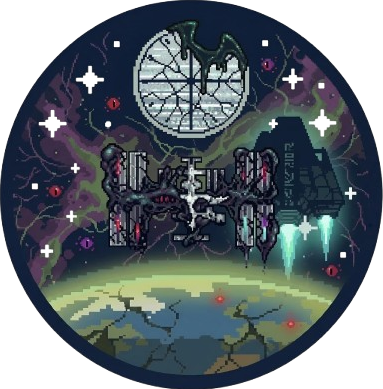
\includegraphics[height=5cm]{icon.png} \\[1cm]
        
        {\large Louay Amara, Hugo Ayaden, Mathis Dos Santos}\\[0.2cm]
        {\large Bastien Lefevre Taugourdeau} \\[0.5cm]
     
        {\large 1 avril 2026}\\
        
        \Huge\href{https://github.com/HugoAyaden/Solitude-408}{GitHub Solitude 408}
    \end{center} 
\end{titlepage}

\newpage

\tableofcontents

\newpage
\section{Introduction}

\textit{Cette introduction présentera le contexte du projet, le concept du jeu ainsi que le plan adopté pour ce compte rendu.} \\

Dans le cadre du projet de fin d'année de L2 Informatique, le présent rapport détaille la conception et le développement de \textit{Solitude 408}. Il s'agit d'un jeu vidéo de type survival horror\footnote{Jeu d'action-aventure centré sur la survie et l'angoisse.} en vue subjective, programmé en langage C et s'appuyant sur les bibliothèques \Gls{sdl2}\cite{bib_sdl2}. S'inspirant de classiques modernes de l'horreur indépendante (comme \acrshort{fnaf}), le jeu invite le joueur à prendre la place d'un gardien de nuit solitaire qui doit faire face à des entités hostiles (le Monstre et le Mimic), pendant qu'il cherche à survivre jusqu'au lever du jour dans une pièce de surveillance, en gérant judicieusement des ressources limitées telles que l'énergie de la batterie, l'éclairage et la fermeture des portes. \\

En première partie, ce document exposera la phase de conception du projet. Elle détaillera le cahier des charges initial fixant les contraintes de développement, ainsi que l'ensemble des fonctionnalités prévues pour offrir l'expérience de jeu souhaitée. \\

Ensuite, l'organisation globale du travail sera abordée. Cette section expliquera la répartition des tâches au sein de l'équipe, le planning prévisionnel mis en place pour respecter les délais, ainsi que les différents outils de travail et de collaboration utilisés pour mener à bien ce développement. \\

La troisième partie, constituant le cœur technique du rapport, se concentrera sur le développement logiciel. Elle expliquera successivement l'architecture de la gestion des menus, la création technique de la carte (génération des cases et salles spéciales) et la production des ressources (audios et images). L'implémentation des mécaniques clés du jeu (batterie, portes, lumières, caméras et intelligence artificielle) sera ensuite analysée. Enfin, la mise en place de l'interface de jeu, incluant les interactions et les transitions visuelles, viendra clore ce volet technique. \\

Enfin, le document s'achèvera sur une présentation des résultats obtenus, suivie d'une conclusion générale dressant le bilan de cette expérience de programmation.

\section{Conception}

    \textit{Dans cette partie seront expliquées les différentes étapes de recherches et analyses des spécificités du projet.}

    \subsection{Cahier des charges}
        Dans le cadre de la formation de L2 Informatique, un projet de fin d’année sous la forme d’un mini jeu développé en langage C est demandé. Celui-ci se fera en groupe de 4 maximum. Le thème du jeu est partiellement libre, seul le feu vert des responsables de la filière L2 Informatique est nécessaire.\\

        Les objectifs principaux du projet sont de permettre aux étudiants de mettre en pratique leurs différents acquis lors de la formation grâce à un projet collectif qui devrait développer l’autonomie et la prise d’initiative des élèves.\\
        
        On notera aussi les objectifs de développement suivants :
        \begin{itemize}
            \item créer et mettre en œuvre des algorithmes,
            \item conduire un projet en petit groupe,
            \item utiliser des outils spécifiques au développement et à la gestion de projet,
            \item développer la communication par le biais d’un travail écrit et d’un oral.\\
        \end{itemize}

        Le projet devra respecter différentes attentes de conception et de développement :
        \begin{itemize}
            \item recherche des règles de jeu et adaptation de celles-ci,
            \item présence d’un \Gls{makefile} élaboré,
            \item gestion de version sur \Gls{github}\cite{bib_github},
            \item création d’une documentation avec \Gls{doxygen}\cite{bib_doxygen},
            \item possibilité de sauvegarder l’état du jeu dans un fichier ainsi que le chargement de celui-ci,
            \item création d’un rapport de 15~20 pages avec \Gls{latex},
            \item mise en place d’une diapositive de présentation pour l’oral avec démo en vidéo.\\
        \end{itemize}

        Le délai du projet s'étend du 13 janvier 2026 au 17 avril 2026, où, le 17 avril, correspond à la date de la soutenance finale. Le rapport devra être définitivement terminé pour le 10 avril 2026 est une version jouable du jeu devra être obligatoire pour la même date.

  \subsection{Fonctionnalités}

    \textit{Cette section détaille les mécaniques de jeu principales ainsi que le déroulement de l'expérience proposée au joueur.} \\

    Le jeu de \textit{Solitude 408} s'articule autour d'une boucle de survie stratégique en temps réel. Isolé dans la salle de surveillance d'une station spatiale en orbite (à 408 km d'altitude), le joueur doit survivre à travers une série de nuits en gérant des ressources limitées face à  des entités hostiles.

    \subsubsection{Boucle de jeu}
    Pour survivre jusqu'au matin, le joueur doit jongler entre différents systèmes de sécurité tout en surveillant constamment son niveau de batterie, qui démarre à 100\%. Atteindre 0\% plonge la station dans l'obscurité totale et signe la fin de la partie. Les fonctionnalités à disposition sont :
    \begin{itemize}
        \item \textbf{Le Moniteur de Caméras :} Outil indispensable pour traquer les entités dans les 9 salles et couloirs numérotées de la station. Son utilisation prolongée produit cependant un bruit électronique susceptible d'attirer certaines menaces.
        \item \textbf{Les Portes et Lumières :} Seuls moyens de défense physique du bureau. Fermer une porte empêche les intrusions, et allumer les lumières des couloirs permet de vérifier les angles morts. Ces actions drainent cependant la batterie de manière significative.
        \item \textbf{Le Blackout (Coupure générale) :} Une mécanique permettant d'éteindre les lumières et d'ouvrir les portes pour se cacher dans le noir total, essentielle pour échapper aux entités sensibles au bruit, au prix d'une vulnérabilité face aux attaques physiques.
    \end{itemize}

    \subsubsection{Gestion des Menaces}
    Le joueur est confronté à deux types d'antagonistes aux comportements opposés, exigeant une attention visuelle et sonore constante :
    \begin{itemize}
        \item \textbf{L'Alien (Le Traqueur) :} Une entité physique issue d'une brèche dans la station. Il est sensible à la lumière (ralenti par le flash des caméras actives) et bloqué par les portes fermées. Son approche est signalée par une augmentation des parasites visuels (effet statique) sur l'écran du joueur.
        \item \textbf{Le Mimic (L'Imitateur) :} Une entité attirée par le bruit du moniteur de caméras. Son approche est trahie par des indices sonores (distorsion vocale au téléphone, grattements dans les murs gauche, mélodies effrayantes). Pour le contrer, le joueur doit impérativement baisser son moniteur et plonger la salle dans le noir total.
    \end{itemize}

    \subsubsection{Déroulement de l'Aventure}
    
    La progression du jeu est structurée autour d'un cycle de 5 nuits (Jours 0 à 4), introduisant progressivement les mécaniques et faisant évoluer la tension narrative :
    \begin{itemize}
        \item \textbf{Jour 0 (Safety) :} Fait office de tutoriel. Le joueur se familiarise avec le cycle des caméras et la disposition des lieux dans un environnement calme. C'est également l'introduction vocale du "Phone Guy", le collègue censé aider le joueur.
        \item \textbf{Jour 1 (Breach) :} L'alarme retentit, signalant une brèche. Introduction de l'Alien. Le joueur apprend à gérer l'équilibre entre sa sécurité et la consommation de sa batterie.
        \item \textbf{Jour 2 (Hunt) :} La vitesse de l'Alien s'accroît, accentuant la menace sur les portes. Les premiers signaux d'alerte narratifs apparaissent (la voix du Phone Guy semble fatiguée, des bruits étranges résonnent dans les murs).
        \item \textbf{Jour 3 (Mimic) :} Point de bascule du scénario. Le joueur découvre que le véritable Phone Guy est mort depuis le début. L'appel en cours ne s'arrête pas et se transforme en mélodie. Le Mimic devient actif, forçant le joueur à alterner entre la défense visuelle (portes contre l'Alien) et la défense furtive (Blackout contre le Mimic).
        \item \textbf{Jour 4 (Solitude) :} Difficulté maximale. Le joueur est livré à lui-même dans une station mourante sans plus aucune aide vocale. L'efficacité énergétique et la maîtrise absolue des mécaniques visuelles et sonores sont vitales pour espérer survivre.
    \end{itemize}

\section{Organisation du projet}
    \subsection{Répartition des tâches}
        
        La répartition des tâches au sein du projet s’est faite naturellement en fonction des compétences et des préférences de chacun. Chaque membre s’est vu attribuer les éléments du projet correspondant le mieux à son domaine de préférence, tout en maintenant une communication régulière pour assurer la cohérence d’ensemble. Par exemple, certains membres se sont concentrés sur la logique de gameplay, l’équilibrage des mécaniques ou encore la création des interfaces et des éléments visuels. Cette répartition a permis d’avancer efficacement.\\
        
        Pour structurer la progression du développement du jeu, deux diagrammes de \Gls{gantt} ont été faits : un prévisionnel en début de projet, puis un second mis à jour régulièrement. Certaines tâches, comme l’intégration de fonctionnalités complexes ont demandé plus de temps que prévu. Par exemple, des problèmes inattendus liés à la gestion des nuits ont rallongé certaines étapes.\\
        
        La comparaison entre les deux diagrammes de \Gls{gantt} met en évidence l’importance d’une planification adaptable. Les réunions régulières ont joué un rôle clé : elles ont permis d’ajuster les priorités, de redistribuer certaines tâches lorsque nécessaire et d’optimiser l’utilisation du temps et des compétences de chacun. Cette organisation flexible a été utile pour mener le projet à bien malgré les imprévus.

    \subsection{Planning prévisionnel}
    \textit{La section suivante présente le découpage du planning prévisionnel.}\\

    Le \href{https://docs.google.com/spreadsheets/d/10BtX8lV49BRHHMKD-WF7gbojdl62evs0IOK-swW39dE/edit?usp=drive_link}{planning prévisionnel} est un diagramme de \Gls{gantt} effectué sur \Gls{google_sheet}. Il comporte les tâches du projet découpées en phases distinctes : initialisation, analyse et spécification, conception, réalisation, recette, exploitation et maintenance.\\
 
    La première phase dite d’initialisation, pose les bases du projet et comporte :
    \begin{itemize}
            \item l'analyse des risques et la mise en place de procédures correctives,
            \item le plan d’assurance qualité,
            \item le plan de développement,
            \item le planning provisionnel et la planification des tâches.\\
    \end{itemize}

    La phase d’analyse et spécification définit ce que doit faire le jeu et les contraintes de celui-ci, les objectifs sont :
    \begin{itemize}
            \item la définition de l'existant et des besoins,
            \item la définition des contraintes techniques et fonctionnelles,
            \item le dossier de tests de validation.\\
    \end{itemize}

    Dans la phase de conception, la structure du jeu y est définie et comporte :
    \begin{itemize}
            \item le maquettage et la définition de l'arborescence du jeu,
            \item le découpage du projet en modules,
            \item le dossier des tests unitaires et d'intégrations.\\
    \end{itemize}

    La phase de réalisation correspond au développement du jeu et de l'application des tests unitaires et d'intégrations.\\

    L'avant-dernière phase intitulée phase de recette est la validation des tests précédents.\\

    Enfin, la phase d'exploitation et maintenance vise la rédaction du dossier d'installation, la correction des anomalies et l'évolution du produit.
    
    \subsection{Outils de travail}
        \textit{Cette partie rassemble les outils de travail utilisés lors du projet et leur rôle dans celui-ci.}\\

        Les différents outils de travail ont été répartis en sept catégories : développement, documentation, gestion, création, environnement, débogage et communication. Les outils sont tous visibles dans le \autoref{tab:outils1} et le \autoref{tab:outils2}.
    Les outils de développement correspondent aux langages utilisés (langage C), aux bibliothèques permettant de simplifier la manipulation d'images, de polices d'écriture, d'audios et des différents matériels informatiques (\Gls{sdl2}, \Gls{sdl2_image}, \Gls{sdl2_ttf}, \Gls{sdl2_mixer}), aux logiciels de compilation (\Gls{gcc}\cite{bib_gcc} et \Gls{make}\cite{bib_make}) et à toutes les \acrshort{ia} génératrices de code redondant (\Gls{github_copilot}).\\
    
    La catégorie documentation représente les outils permettant la génération de commentaires (\Gls{github_copilot}), de documentation logicielle (\Gls{doxygen}) et la création de livrables (\Gls{google_suite} et \Gls{latex}).\\
    
    Les outils catégorisés de "Gestion" peuvent permettre le versionnage du code (\Gls{git}\cite{bib_git}), de stocker plusieurs itérations du code (\Gls{github}), stocker des fichiers (\Gls{google_drive}\cite{bib_drive}) et de comparer et fusionner du code (\Gls{git}).\\

    Toutes les applications mentionnées dans la section "Création" peuvent produire des rendus 3D (\Gls{blender}\cite{bib_blender}), du traitement d'images (\Gls{gimp}\cite{bib_gimp}), du traitement audio (\Gls{audacity}\cite{bib_audacity}) et la génération de contenu (\Gls{gemini}\cite{bib_gemini}).\\

    Les environnements sont les systèmes d'exploitation utilisés lors du développement (Windows, Mac OS, Linux), les \acrshort{ide} (\Gls{vs_code}\cite{bib_vscode}) et les plateformes de distribution et de développement logiciel (\Gls{msys2}\cite{bib_msys2}).\\

    Le débogage du jeu est effectué avec des logiciels de débogage de mémoire (\Gls{valgrind}\cite{bib_valgrind} pour Linux/MacOS et \Gls{dr_memory}\cite{bib_dr_memory} pour Windows), ainsi que d'un débogueur général permettant l'arrêt et la reprise du code ainsi que de visualiser le contenu des variables (\Gls{gdb}\cite{bib_gdb}).\\

    Enfin, pour la communication, l'équipe échange par le biais de logiciel de discussion instantanée (\Gls{discord}\cite{bib_discord}), courrier électronique (Mail \acrlong{lmu}). Toute communication des tâches est inscrite sur le planning réel \Gls{gantt} (\Gls{google_suite}) et par logiciel de gestion de développement (\Gls{github}).
            \begin{table}[h!]
            \centering
            \begin{tabular}{|c|c|c|c|}
                \hline
                Développement        & Documentation        & Gestion             & Création       \\
                \hline
                Langage C            & \Gls{doxygen}        & \Gls{github}        & \Gls{blender}  \\
                \Gls{sdl2}           & \Gls{google_suite}   & \Gls{git}           & \Gls{gimp}     \\
                \Gls{sdl2_ttf}       & \Gls{latex}          & \Gls{google_drive}  & \Gls{audacity} \\
                \Gls{sdl2_image}     & \Gls{github_copilot} &                     & \Gls{gemini}   \\
                \Gls{sdl2_mixer}     &                      &                     &                \\
                \Gls{gcc}            &                      &                     &                \\
                \Gls{make}           &                      &                     &                \\
                \Gls{github_copilot} &                      &                     &                \\
                \hline
            \end{tabular}
            \caption{Outils de travail}
            \label{tab:outils1}
        \end{table}

        \begin{table}[h!]
            \centering
            \begin{tabular}{|c|c|c|c|c|}
                \hline
                Environnement   & Débogage          & Communication       \\
                \hline
                Linux           & \Gls{gdb}         & \Gls{discord}             \\
                Mac OS          & \Gls{dr_memory}   & \Gls{github}              \\
                Windows         & \Gls{valgrind}    & \Gls{google_suite}         \\
                \Gls{msys2}     &                   & Mail \acrshort{lmu} \\
                \Gls{vs_code}   &                   &                     \\
                \hline
            \end{tabular}
            \caption{Outils de travail (suite)}
            \label{tab:outils2}
        \end{table}

\section{Développement}
\subsection{Gestion des menus}

La gestion des interfaces repose sur une architecture de machine à états. Cette structure garantit une navigation fluide entre le menu principal, les paramètres et les crédits tout en évitant les erreurs d'affichage. \\

\begin{itemize}
    \item \textbf{Logique de fonctionnement :} L'organisation du code s'appuie sur une énumération nommée Game State. Elle définit précisément l'état du programme (STATE\_MENU, STATE\_SETTINGS, STATE\_CREDITS) à chaque instant. L'utilisation d'une variable pour l'état actuel et d'une autre pour l'état cible (Next) permet d'anticiper les changements d'écran. Cette méthode empêche les conflits entre les interfaces et permet de délimiter clairement le rendu visuel et les actions de l'utilisateur. \\

    \item \textbf{Organisation du code :} La machine à états permet de compartimenter le programme. Lorsqu'un écran est actif, seuls les événements et les images qui lui correspondent sont traités. Cela évite, par exemple, qu'un clic sur le menu principal n'active par erreur un bouton des paramètres. Cette séparation rend le système stable et facilite les futures modifications. \\

    \item \textbf{Aspect Visuel :} Le projet adopte une esthétique cinématographique (Figure \ref{fig:menu})inspirée de productions modernes. Les boutons sont alignés sur la gauche avec un texte agrandi (facteur d'échelle de 1,25x) afin de mieux remplir l'espace et de renforcer l'immersion dès le lancement. \\

    \item \textbf{Système de transition :} Un effet visuel de "glitch" renforce l'identité "Horreur" du jeu lors des changements d'écran. Cette transition est pilotée par une variable flottante (Progress) allant de 0.0 à 1.0. Lorsque le "glitch" atteint son opacité maximale (0.5), le programme effectue le basculement invisible entre les deux états du jeu, garantissant une continuité parfaite pour l'utilisateur. Ce système est synchronisé avec l'audio : le bruit blanc de la transition s'accompagne d'une baisse progressive du volume (fade-out) de la musique du menu, garantissant une cohérence sonore. \\

    \item \textbf{Optimisation et fluidité :} Afin d'assurer une transition parfaitement fluide vers le cœur du jeu, les ressources lourdes (textures, effets sonores) sont préchargées en mémoire vive (RAM) au lancement de l'exécutable. Cette architecture logicielle supprime les temps de chargement matériels lors du lancement d'une nouvelle partie. Ainsi, la transition visuelle s'exécute instantanément sans jamais figer l'écran ou interrompre le thread principal.
\end{itemize}

\begin{figure}[htbp]
    \centering
    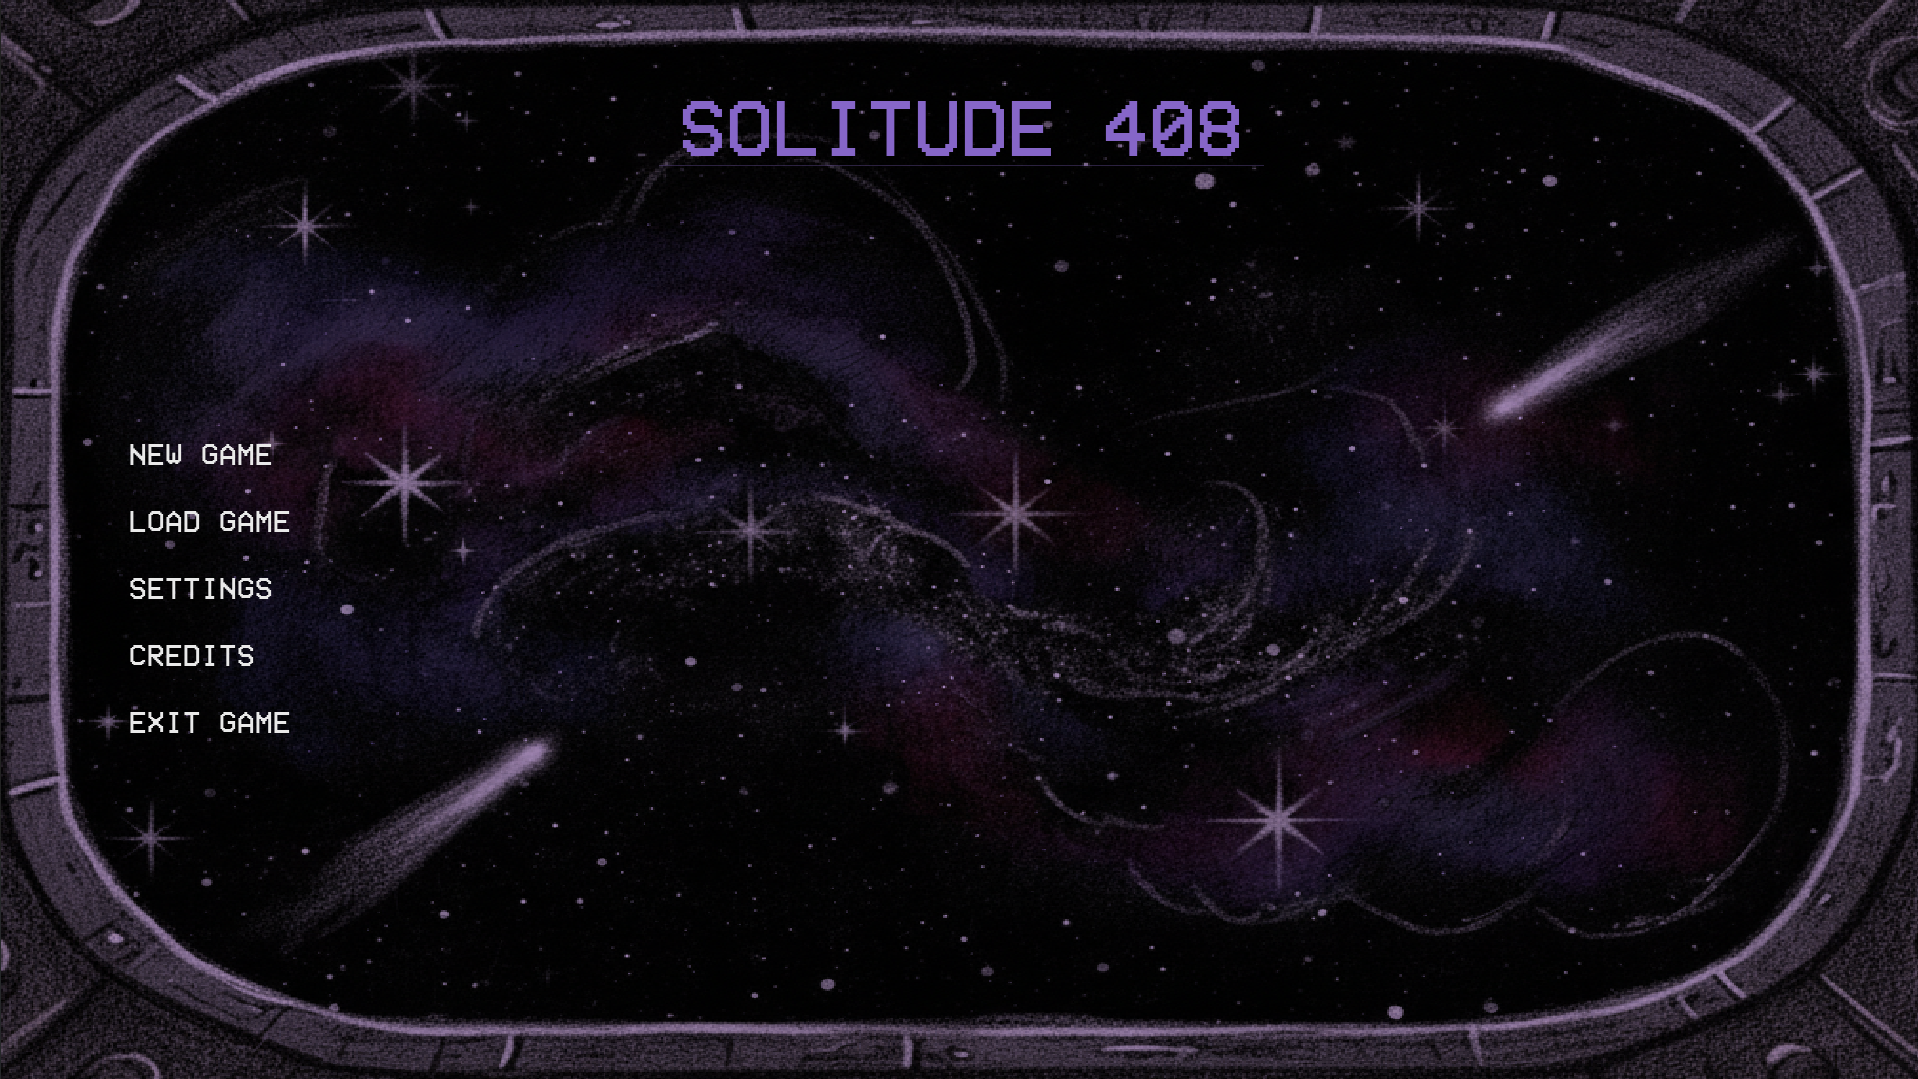
\includegraphics[width=1\linewidth]{menu.PNG}
    \caption{Menu principal du jeu.}
    \label{fig:menu}
\end{figure}

\subsection{Création de la carte}
\textit{Dans cette partie, nous développerons tout ce qui touche au développement du jeu cartes, ressources, caméras et autres éléments de gameplay.}

\subsubsection{Cases}

Le jeu se passe dans un vaisseau bloqué dans l'espace, la \hyperref[fig:carte]{carte} doit donc être crédible et à la fois utile au gameplay.\\La carte est une matrice de 3x5 (Figure \ref{fig:matrice}) \textit{case\_t} cases dont chacune possède 7 paramètres :

\begin{itemize}
    \item numéro de caméra,
    \item lumière,
    \item accès,
    \item voisin haut,
    \item voisin bas,
    \item voisin gauche,
    \item voisin droit.\\
\end{itemize}

Voyons les un par un:
\begin{itemize}
    \item\textbf{Numéro de caméra \textit{(entier) :}} C'est le cœur de la localisation puisqu'il donne la position de chaque entité en temps réel. Il est donc énormément utilisé pour la détection des attaques ou la gestion des déplacements.
    \item\textbf{lumière \textit{(booléen) :}} Surtout utile pour le joueur et le mimique, il permet de savoir si la lumière du bureau est allumée.
    \item\textbf{accès \textit{(booléen) :}} Permet de détecter si le monstre peut ou ne peut pas accéder à certaines salles.
    \item\textbf{Voisins \textit{(case\_t) :}} Donne pour chaque case qui est sa voisine (pour une case sans voisin elle est égale à null).\\
\end{itemize}

De plus, des murs sont présents au sein de la carte pour rendre les déplacements du monstre plus organique et permettre une lecture du jeu encore plus technique pour les joueurs qui s'investiront dessus.

\begin{figure}[htbp]
    \centering
    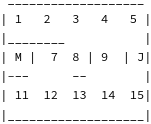
\includegraphics[width=0.35\linewidth]{matrice.png}
    \caption{Matrice du jeu avec les murs.}
    \label{fig:matrice}
\end{figure}

\subsubsection{Salles spéciales}

Enfin, cette carte comporte aussi 2 cases spéciales :

\begin{itemize}
    \item la salle du \textbf{Joueur},
    \item la salle du \textbf{Mimique}.\\
\end{itemize}

Ces salles se trouvent sur la ligne du milieu aux extrémités droites et gauches de la matrice. La salle du joueur est placée ici pour avoir deux entrées droite et gauche, desquelles le monstre peut arriver à tout moment.\\

Quant à la salle du mimique, pour des raisons d'histoire elle est située à l'opposé du joueur, c'est comme son nom l'indique le point d'apparition du monstre à partir de la nuit 2.\\

La salle du joueur est quant à elle le cœur du gameplay puisque le joueur s'y trouve en permanence. Elle possède 2 portes (une à gauche et une à droite) et deux lumières (de même) ainsi qu'un moniteur qui permet d'accéder aux caméras.

\subsection{Création des ressources}
\subsubsection{Création des audios}

La conception de l'environnement sonore s'est articulée autour de deux axes principaux afin de renforcer l'immersion et de soutenir l'identité horrifique du projet. \\

D'une part, une musique originale a été intégralement composée et enregistrée à la guitare. Ce thème musical est utilisé pour habiller l'interface du menu principal ainsi que la séquence de crédits de fin. Ces musiques ont pour but de créer une ambiance angoissante qui correspond parfaitement au thème du jeu : la solitude dans l'espace \\

D'autre part, la conception du \textit{sound design} en jeu (l'ambiance sonore de la station, les interactions avec l'interface, les clics de boutons ou encore les lourds bruits de fermeture des portes) a nécessité une approche différente. Afin de garantir une immersion réaliste, le projet s'est appuyé sur la banque de sons participative freesound.org \cite{bib_freesound} pour assurer une sélection d'effets sonores professionnels et libres de droits afin d'optimiser l'expérience du joueur.

\newpage
\subsubsection{Création des images}

Les images sont créées grâce à Blender. Elles sont pré-rendues en 3D et chargées à l'aide de la fonction \textbf{afficher()} qui choisit le fond d'écran en fonction de l'état du jeu.\\

Chaque caméra est rendue dès que le jeu détecte l'activation du bouton caméra, chaque caméra doit posséder 4 images différentes pour : vide, avec le monstre, avec le mimique, avec le monstre et le mimique.

\subsection{Mise en place des mécaniques}
\subsubsection{Batterie, Portes et Lumières}

Dans le cadre du développement du jeu, un ensemble de mécaniques interconnectées a été mis en place afin de créer une tension constante pour le joueur. Parmi ces systèmes, la gestion de la batterie, le contrôle des portes et l’utilisation des lumières constituent le cœur du gameplay. Ces mécaniques ont été conçues pour obliger le joueur à effectuer des choix stratégiques en temps réel. Cette section décrit leur conception, leur rôle dans le jeu ainsi que leur implémentation technique.\\ 

La batterie représente la quantité d’énergie disponible pour alimenter les différents dispositifs du bureau. Elle constitue la ressource principale du joueur et conditionne directement sa capacité à survivre, elle impose une contrainte temporelle et stratégique. En effet, le joueur doit survivre pendant une nuit sans épuiser totalement la batterie. Une batterie vide entraîne l’incapacité d’utiliser les systèmes de défense, rendant le joueur vulnérable aux monstres. Ce système introduit une notion de gestion des ressources, où chaque action a un coût. Le joueur doit donc anticiper ses besoins et éviter toute consommation excessive. La batterie est modélisée par une variable numérique représentant un pourcentage d’énergie restante. Cette valeur est décrémentée progressivement au cours du temps à l’aide d’un système de mise à jour (boucle principale du jeu).\\

La consommation d’énergie dépend de l’état des autres systèmes :
\begin{itemize}
    \item consommation de base,
    \item augmentation lorsque des portes sont fermées,
    \item augmentation lorsque des lumières sont allumées.
\end{itemize}
\newpage
Un système de calcul permet d’ajuster la vitesse de décharge en fonction du nombre d’éléments actifs. Cela permet une gestion fine de la difficulté. Les portes constituent le principal moyen de protection du joueur contre les monstres. Chaque porte peut être ouverte ou fermée. Lorsqu’elle est fermée, elle empêche le monstre d’entrer dans le bureau, assurant ainsi la sécurité du joueur.\\

Cependant, ce mécanisme introduit un compromis important : une porte fermée consomme de l’énergie en continu. Le joueur doit donc décider du meilleur moment pour fermer ou ouvrir une porte. Ce système crée une tension constante, car une utilisation excessive des portes peut entraîner une décharge rapide de la batterie. Les portes sont représentées par des variables d’état (ouvertes ou fermées). Leur état peut être modifié via les boutons mis à disposition.\\

Lorsqu’une porte est fermée (Figure \ref{fig:porte}) :
\begin{itemize}
    \item son état est mis à jour,
    \item une consommation d’énergie supplémentaire est appliquée,
    \item l'écran est mis à jour, la porte se ferme.\\
\end{itemize}

\begin{figure}[htbp]
    \centering
    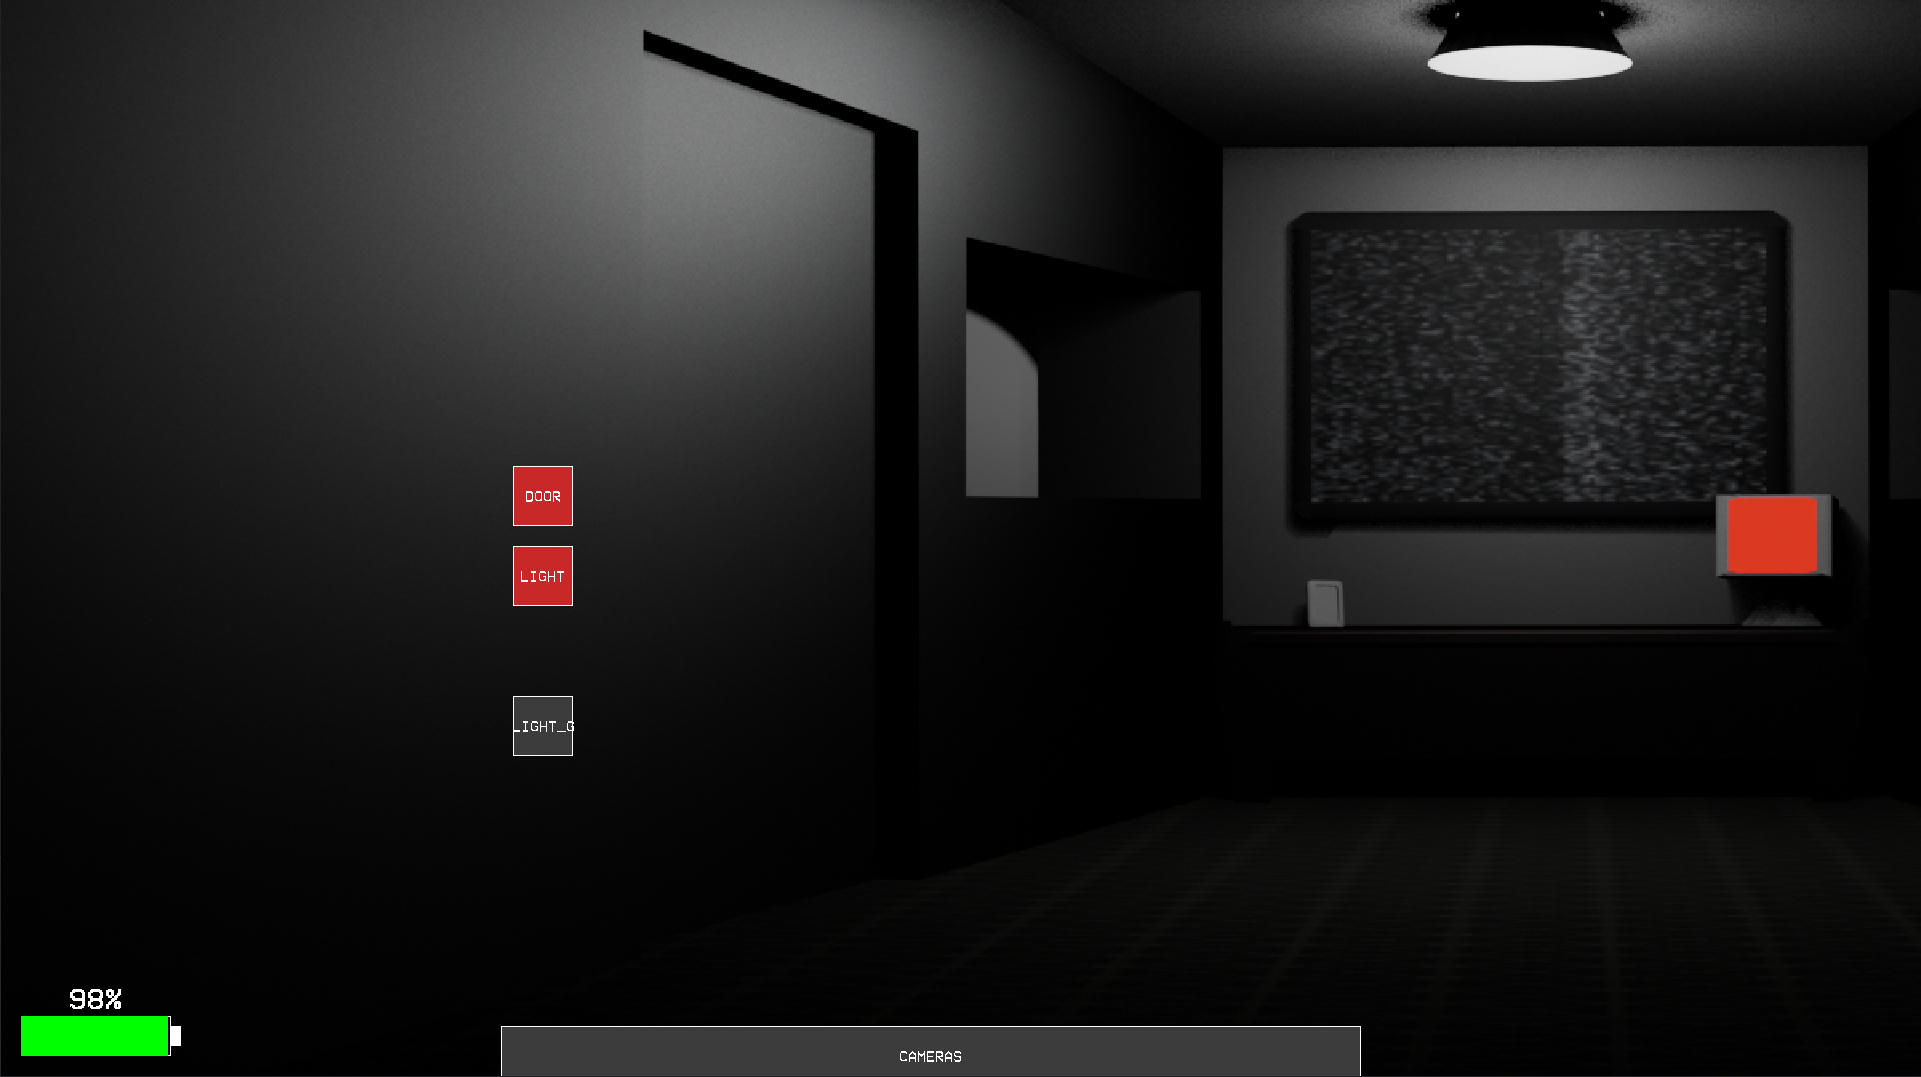
\includegraphics[width=1\linewidth]{porte.PNG}
    \caption{Exemple avec la porte gauche fermée.}
    \label{fig:porte}
\end{figure}
Le système est intégré dans la boucle principale du jeu afin de garantir une mise à jour en temps réel. Les lumières permettent au joueur d’observer la présence des monstres. Contrairement aux portes, les lumières n’offrent pas de protection directe. Leur rôle est informatif : elles permettent au joueur de prendre des décisions. 
\newpage
Par exemple, le joueur peut activer une lumière pour vérifier si le monstre est présent avant de fermer une porte. Cela évite une consommation inutile d’énergie. Cependant, leur utilisation a également un coût énergétique, ce qui empêche le joueur de les utiliser en permanence.
Les lumières sont activées de manière temporaire via une interaction utilisateur.\\ 

Lorsqu’elles sont actives :
\begin{itemize}
    \item une zone spécifique est éclairée à l’écran,
    \item un indicateur visuel est affiché,
    \item une consommation d’énergie est appliquée.\\
\end{itemize}

La batterie agit comme une contrainte globale, limitant l’utilisation des portes et des lumières. Les portes assurent la sécurité mais consomment en continu, tandis que les lumières permettent d’optimiser leur utilisation en fournissant des informations.\\

Cette interaction crée une boucle de gameplay où le joueur doit constamment équilibrer sécurité et économie d’énergie. L’ensemble de ces mécaniques contribue à instaurer une tension permanente. Le joueur est confronté à des choix difficiles avec des conséquences immédiates. La gestion de la batterie introduit une pression temporelle, les portes créent une sécurité limitée, et les lumières apportent une aide stratégique au prix d’une surconsommation. Ainsi, le gameplay repose sur un équilibre fragile entre prise de risque et prudence, ce qui renforce l’immersion et l’engagement du joueur.
\subsubsection{Caméras}

\begin{figure}[htbp]
    \centering
    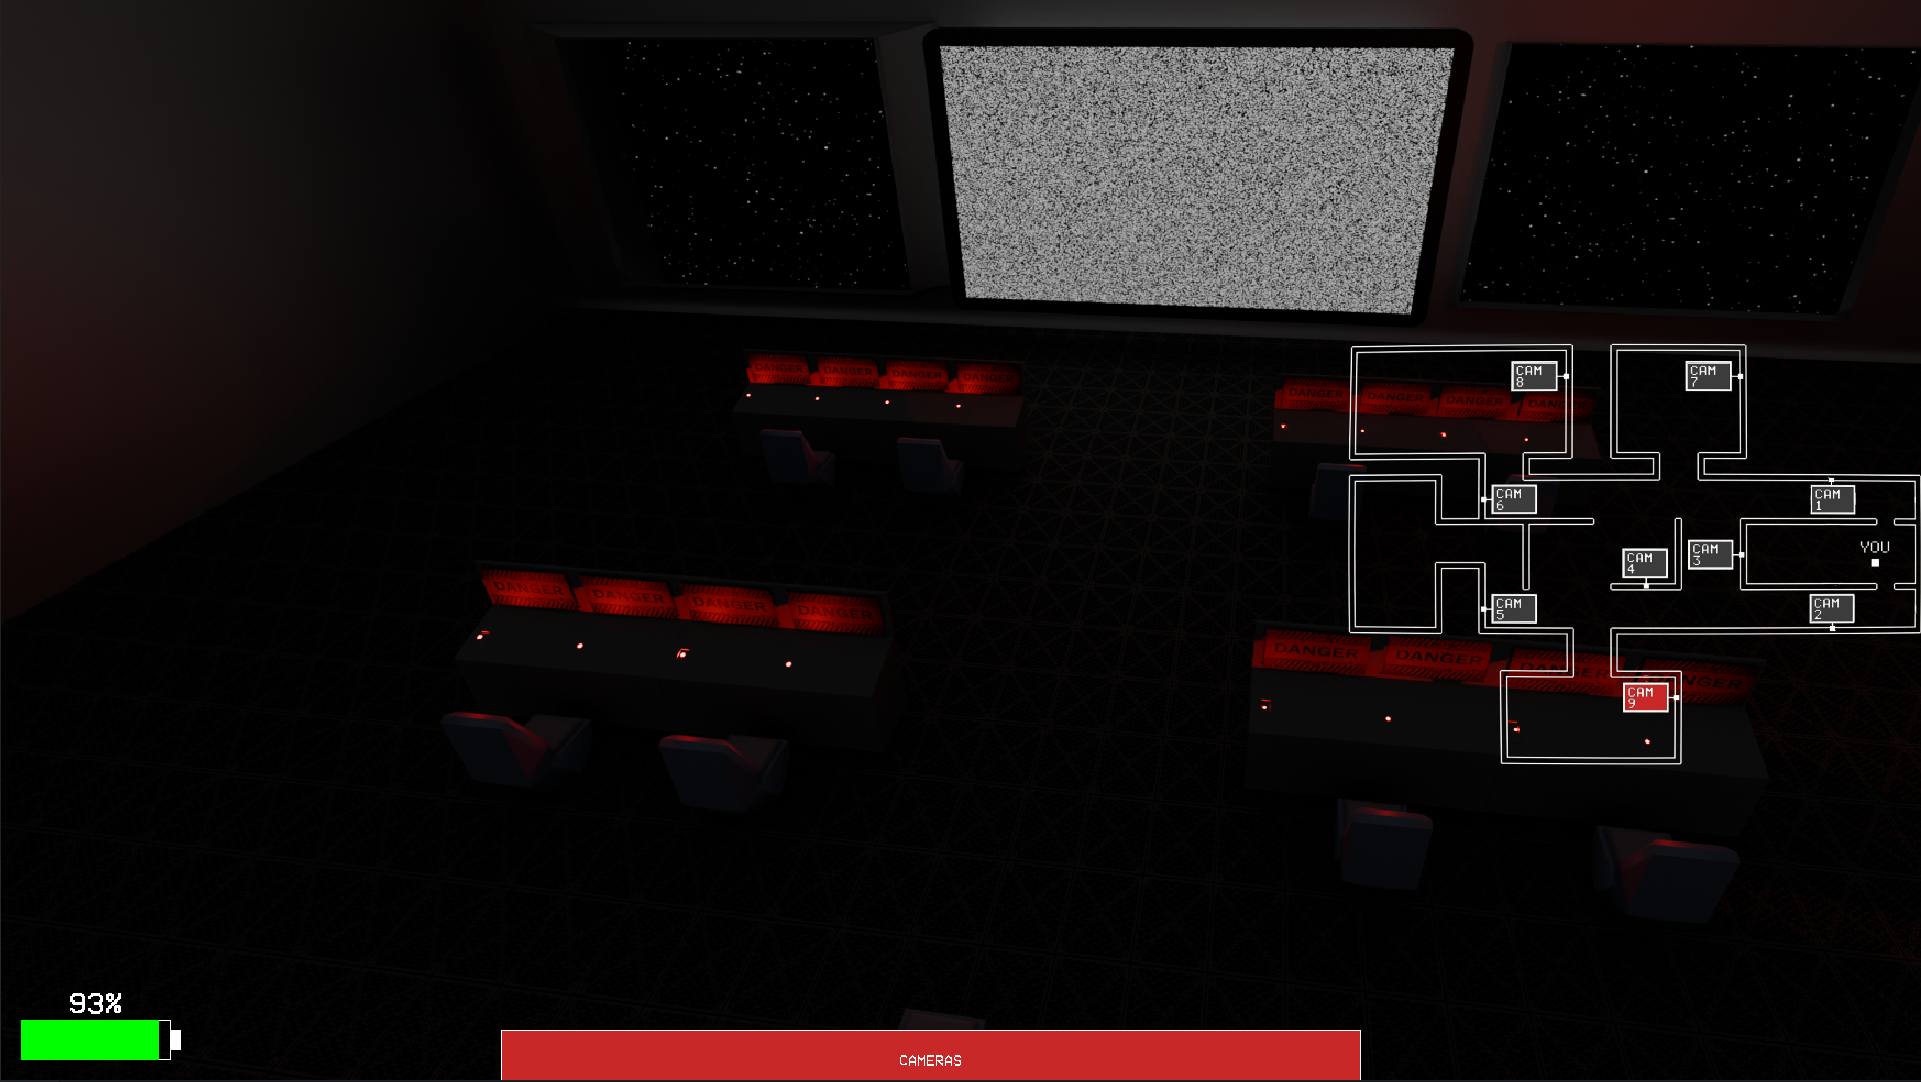
\includegraphics[width=0.9\linewidth]{cam.PNG}
    \caption{Interface des caméras dans le jeu.}
    \label{fig:cam}
\end{figure}

Les caméras (Figure \ref{fig:cam}) sont un élément central du gameplay, il fallait donc réfléchir à une manière pratique, visible et rapide d'y accéder puisque le jeu peut basculer en une seconde. Le choix a donc été de placer le moniteur en bas de l'écran en permanence afin qu'il soit accessible rapidement de n'importe où et de rendre le bouton vraiment large afin que le joueur ne puisse pas rater son action sous le coup du stress. Le moniteur est aussi placé en bas de l'écran afin de ne pas gêner la vision du joueur dans son bureau.\\

La gestion des caméras est faite d'un pointeur sur une cases\_t à la fois. Le jeu en lit les valeurs et vérifie si parmi les monstres, aucun ne se trouve sur la caméra. en fonction des données, il change l'affichage.\\

Les caméras possèdent une carte pour permettre au joueur de savoir où se trouve l'endroit qu'il regarde et se figurer si le monstre est loin ou non. Le choix de mettre des caméras juste devant les portes permet au joueur de pouvoir réagir en cas d'urgence sans avoir à constamment retirer les caméras pour savoir si le monstre ne s'est pas glissé derrière sa porte sans qu'il ne s'en rende compte.\\



\subsubsection{Intelligence artificielle}

Le jeu possède deux \acrshort{ia}, la première est celle qui nous attaque du début à la fin du jeu, c'est le "monstre". Il apparaît soit dans la case 1 de la \hyperref[fig:carte]{carte} soit dans la case 11, son schéma d'attaque change entre les nuits : 
\begin{itemize}

    \item\textbf{NUIT 1 : }le monstre se déplace aléatoirement à travers la carte. Il fait un choix entre 4 directions au hasard (HAUT, BAS, GAUCHE, DROITE), si cette destination est accessible il y va sinon il ne bouge pas.
    Ses chances de déplacement sont faibles (10\%) afin de laisser au joueur le temps de découvrir son environnement et le fonctionnement du jeu.\\
    
    \item\textbf{NUIT 2 : }le monstre utilise un algorithme se servant d'une file pour trouver le chemin le plus court jusqu'au joueur appelé "\acrshort{bfs} \cite{bib_bfs1} \cite{bib_bfs2}" complexité O(N)).Cet algorithme n'est pas le plus optimisé en règle générale dans des grands tableaux ou graphiques, on préfère utiliser le "\acrshort{dfs}\cite{bib_dfs}" complexité O(N)), mais dans des petits espaces comme la matrice du jeu, il est le plus efficace des deux pour trouver un point précis.
    Ses chances de déplacement sont moyennes, 35\% de chance de se déplacer de manière optimisée (vers le joueur), sinon le monstre utilise le même système de déplacement qu'à la nuit 1 ; il devient plus agressif et le joueur peut déjà commencer à avoir du mal à le repousser.\\
    
    \item\textbf{NUIT 3 : }à cette nuit, le monstre n'utilise presque exclusivement que le déplacement optimisé (70\% de chances), il est donc extrêmement agressif et demande au joueur de savoir gérer efficacement sa batterie.
    C'est à cette nuit qu'est implémenté le mimique, le second monstre du jeu.\\
\end{itemize}

    Le Mimique a un fonctionnement très différent du monstre puisqu'il se téléporte. Il est incapable de se téléporter directement sur le joueur et relance au hasard une case sur laquelle aller si la précédente était celle du joueur. La seule manière de détecter le mimique est de le voir sur les caméras puisqu'il n’apparaîtra jamais au niveau des portes afin d'obliger le joueur à utiliser son moniteur. On sait que le mimique s'est déplacé avec le rire qu'il produit, ce qui indique au joueur de vite regarder ses caméras.\\

    Le joueur peut contrer les ennemis des façons suivantes :
    \begin{itemize}
        \item\textbf{Monstre:} Pour l'empêcher d'entrer, le joueur devra uniquement se servir des portes mises à sa disposition et dès que le son de frappement contre la porte est entendu, cela signifie que le monstre est retourné à son point d'apparition.\\
        
        \item\textbf{Mimique:} Pour le mimique, les portes ne sont pas un problème et il peut aisément les traverser, le joueur devra donc utiliser une autre manière. Un bouton spécial existe celui des lumières générales qui éteignent toutes les lampes et ouvrent les portes. Le mimique est sensible à la lumière et si le joueur n'en utilise plus, le mimique ne fera que passer. La lumière de l'ordinateur en face du joueur reste allumée afin que l'utilisateur ne pense pas qu'un problème est survenu en appuyant sur ce bouton et que le jeu a cessé de fonctionner.\\ Un son de déception est entendu lorsque le mimique rate son attaque et réapparaît à la case M de la \hyperref[fig:carte]{carte}. Le monstre peut néanmoins entrer lorsque le bouton des lumières générales est activé puisque le courant est coupé et les portes ouvertes, le joueur doit donc faire preuve d'anticipation pour vite refermer la porte si le monstre est proche. \\Dans tous les cas, le mimique attaquera avant le monstre afin de laisser au joueur une chance de s'en sortir si les deux monstres attaquent en même temps.
    \end{itemize}
    
\newpage
\subsection{Interface de jeu}

\subsubsection{Crédit et transitions}
Les crédits représentent l’ensemble des personnes ayant participé au développement du projet. Leur affichage permet d’identifier clairement les rôles et les contributions de chacun. Cette section intervient à la fin du jeu et est disponible depuis le menu.\\

D’un point de vue technique, les crédits sont implémentés sous la forme d’une liste de chaînes de caractères, affichées dynamiquement à l’écran. Un défilement vertical est utilisé afin de reproduire un effet cinématographique, facilitant la lecture tout en apportant une dimension esthétique. La vitesse de défilement, la taille du texte et le centrage sont des paramètres ajustés afin d’assurer une lisibilité optimale.\\

Les transitions, quant à elles, permettent de relier les différentes phases du jeu de manière fluide. Elles sont utilisées lors du passage d’une nuit à la suivante. Leur rôle est d’indiquer visuellement au joueur un changement de nuit, tout en évitant une rupture brutale dans l’affichage. Une animation spécifique est mise en place pour symboliser cette progression, par exemple par un fondu et un affichage progressif. Ce type de transition renforce l’immersion et contribue à une meilleure compréhension de l’avancement dans le jeu pour le joueur.

\subsubsection{Interactions}
Le joueur peut interagir avec les différents éléments du jeu seulement avec la souris. Cela rend le jeu simple de prise en main et donc, intuitif.\\

Dans le cas du menu principal, le joueur peut démarrer ou charger une partie avec les boutons NEW GAME, LOAD GAME. Il peut quitter le jeu par le bouton EXIT GAME, voir les crédits avec CREDITS. Enfin il est possible de modifier les paramètres de jeu en allant dans SETTINGS. Chacun de ces boutons est activable par le clique gauche de la souris.\\

Les paramètres de jeu sont modifiables grâce aux barres de défilement (MASTER VOLUME, MUSIQUE et BRIGHTNESS). Il est possible de changer la résolution (RESOLUTION) et le format de celle-ci(SCREEN MODE). Le joueur peut sauvegarder ses paramètres avec SAVE ou ne pas les sauvegarder en cliquant sur BACK.
\newpage
Lors d'une partie, le joueur peut interagir avec le monde et déplacer la caméra de jeu de gauche à droite. Pour cela, il doit placer son curseur à 5\% du bord de la fenêtre de jeu (gauche ou droite). Déplacer la caméra permet d'afficher les boutons de porte et de lumières ainsi que d'avoir une vision parfaite sur l'une des deux portes.\\

Enfin, le joueur a la possibilité d'afficher une mini-carte des caméras avec le bouton CAMERAS en bas de la fenêtre de jeu. Le joueur a ainsi la possibilité de choisir d'afficher l'une des neuf caméras de jeu. Pour cela il lui suffit d'appuyer sur n'importe quelle caméra de la mini-carte.\\

Chaque caméra défile automatiquement de gauche à droite sans intervention du joueur.

\section{Résultats et conclusion}

Le résultat final du jeu implémente en majeure partie les fonctionnalités prévues. Cependant, il reste toujours un travail de balance du gameplay. Effectivement, il est difficile d'estimer un ratio temps de batterie/évènements de jeu sans avoir effectué au préalable plusieurs parties de jeu et ceux, dans chaque nuit de jeu.\\

En termes de respect du planning provisionnel, celui-ci n'a pas été respecté entièrement. Outre le non-respect du temps de chaque tâche, les phases d'analyse et spécification ainsi que de conception n'ont pas été complétées entièrement à cause de précipitation. Heureusement, l'équipe étant communicative et partageant la même vision, la phase de réalisation, phase la plus importante, a été réalisée sans encombre.\\

Ce projet a permis à chacun de découvrir de nouveaux outils de travail pour le développement et cela, tout en nous entraidant les uns et les autres créant un partage des connaissances entre tous. De plus, étant un premier projet de développement en équipe, nous avons pu acquérir une vision nouvelle du développement.

\newpage

\section{Bibliographie}

    \begin{thebibliography}{99}
        \bibitem{bib_blender} \textbf{Blender :} \url{https://www.blender.org/}
        \bibitem{bib_gimp}\textbf{Gimp :}\url{https://www.gimp.org/}
        \bibitem{bib_github}\textbf{GitHub :}\url{https://github.com/}
        \bibitem{bib_git}\textbf{Git :}\url{https://git-scm.com/}
        \bibitem{bib_gemini}\textbf{Gemini :}\url{https://gemini.google.com/}
        \bibitem{bib_drive}\textbf{Google Drive :}\url{https://drive.google.com/}
        \bibitem{bib_valgrind}\textbf{Valgrind :}\url{https://valgrind.org/}
        \bibitem{bib_dr_memory}\textbf{Dr.Memory :}\url{https://drmemory.org/}
        \bibitem{bib_gdb}\textbf{GDB :}\url{https://www.sourceware.org/gdb/}
        \bibitem{bib_audacity}\textbf{Audacity :}\url{https://www.audacityteam.org/}
        \bibitem{bib_vscode}\textbf{VS Code :}\url{https://code.visualstudio.com/}
        \bibitem{bib_msys2}\textbf{MSYS2 :}\url{https://www.msys2.org/}
        \bibitem{bib_sdl2}\textbf{SDL2 :}\url{https://www.libsdl.org/}
        \bibitem{bib_make}\textbf{Make :}\url{https://www.gnu.org/software/make/}
        \bibitem{bib_gcc}\textbf{GCC :}\url{https://gcc.gnu.org/}
        \bibitem{bib_discord}\textbf{Discord :}\url{https://discord.com/}
        \bibitem{bib_doxygen}\textbf{Doxygen :}\url{https://www.doxygen.nl/index.html}
        \bibitem{bib_freesound} \textbf{Freesound.org :} \url{https://freesound.org/}
        \bibitem{bib_bfs1}\textbf{GeeksforGeeks :} Implémentation de l'algorithme \acrshort{bfs} en C.\\\url{https://www.geeksforgeeks.org/c/c-program-for-breadth-first-search-or-bfs-for-a-graph/}
        \bibitem{bib_bfs2}\textbf{Wikipédia :} Algorithme de parcours en largeur (\acrshort{bfs}).\\\url{https://fr.wikipedia.org/wiki/Algorithme_de_parcours_en_largeur}
        \bibitem{bib_dfs}\textbf{Wikipédia :} Algorithme de parcours en profondeur\\\url{https://fr.wikipedia.org/wiki/Algorithme_de_parcours_en_profondeur}
    \end{thebibliography}
    \newpage
    \printglossary[type=\acronymtype]
    \printglossary
\newpage
\section{Annexes}
\subsection*{Débogage avec GDB}
\begin{figure}[htbp]
    \centering
    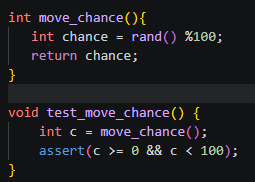
\includegraphics[width=0.5\linewidth]{debug1.PNG}
    \caption{Fonction de test pour savoir si la chance de mouvement d'un monste est bien toujours entre 0 et 99.}
\end{figure}
\begin{figure}[htbp]
    \centering
    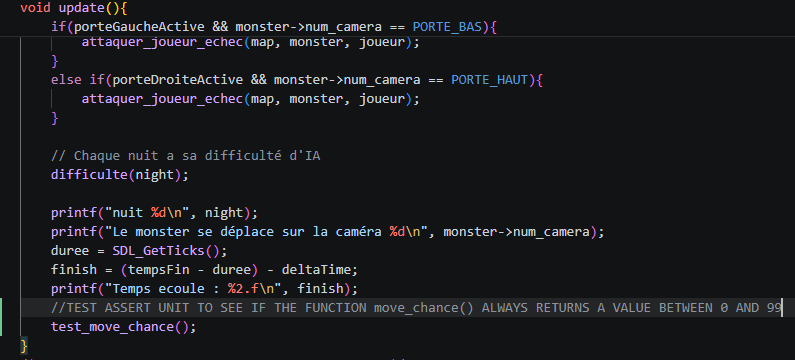
\includegraphics[width=1\linewidth]{debug2.PNG}
    \caption{Application de la fonction de test dans la fonction update() dans le game\_core.c.}
\end{figure}
\begin{figure}[htbp]
    \centering
    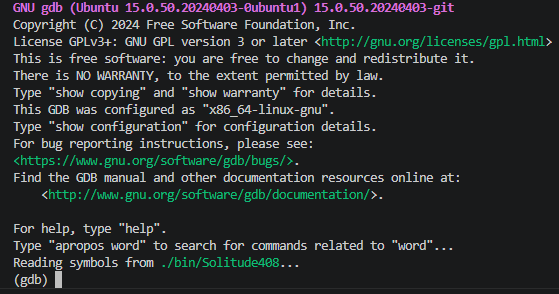
\includegraphics[width=1\linewidth]{debug3.PNG}
    \caption{Appel de GDB.}
\end{figure}
\begin{figure}[htbp]
    \centering
    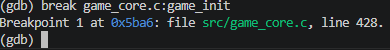
\includegraphics[width=1\linewidth]{debug4.PNG}
    \caption{Mise en place d'un point d'arrêt ligne 428.}
\end{figure}
\begin{figure}[htbp]
    \centering
    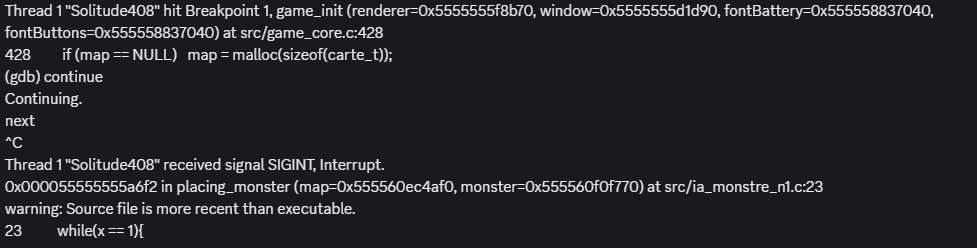
\includegraphics[width=1\linewidth]{debug5.PNG}
    \caption{Log final, boucle infinie dans le fichier ia\_monstre\_n1.c (corrigé).}
\end{figure}

\clearpage 

\end{document}